\documentclass{sig-alternate}

\begin{document}
	\title{CSCI-620 Data Mining with the Airbnb Dataset}
	\subtitle{[Exploring and Mining the dataset of NY Airbnbs]}
	
	\numberofauthors{4}
	\author
	{
		\alignauthor
		Aishwarya Rao
		\email{ar2711@rit.edu}
		\alignauthor
		Apurav Khare
		\email{ak2816@rit.edu}
		\and
		\alignauthor
		Martin Qian
		\email{jq3513@rit.edu}
		\alignauthor
		Prateek Kalasannavar
		\email{pk6685@rit.edu}
	}
	
	\maketitle
	\begin{abstract}
		
		The project aims to create a prediction model on the New York Airbnb Dataset that is capable of predicting which price group a particular house falls into. The approach we use is to build a classification model (such as decision tree) to predict a discrete version of the price (For instance, expensive vs cheap). One of the deliverable this project will include is determining what factors affect the price.   
		
	\end{abstract}

	
	\section{The Data Mining task}
	As mentioned in the previous phase, the data mining task selected was to build a classification model that is capable of predicting the price group a listing would fall into.
	
	\subsection{Targeted Knowledge}
	This data mining task is based on a number of factors. One, a model capable of predicting the price of a new listing has real-world applications. A landlord looking to put up a listing for a new house in New York would be able to use this model to determine the expected range of prices for his house and price it accordingly to make the most profit. Two, the exploration of the dataset revealed that there are a number of attributes in the data that correlate to the price. This indicates that these attributes do help determine the price and validates our hypothesis that the price can be predicted reasonably well by a data mining algorithm. 
	
	\section{Data Exploration and visualization}
	Correlation plots were plotted on attributes against the price to see how they impact it. As a starting point, the attributes that have business meaning in the context of the data are used to plot the correlation plots. These attributes are: "neighbourhood", "neighbourhood\_group", "room\_type", "minimum\_nights", and "availability\_365".\\
	Following are the notable observations:
	\begin{enumerate}
		\item The price of an Airbnb listing varies by the neighbourhood group that it is in. As observed from the correlation plot, the prices of the Airbnb listings in Brooklyn and Manhattan are relatively higher than those in Broknx, Queens, and Staten Island, with the listings in Staten Island being the least priced.
		Figures \ref{neighborhood_grp_corr} depicts these result.
		\begin{figure}[ht]
			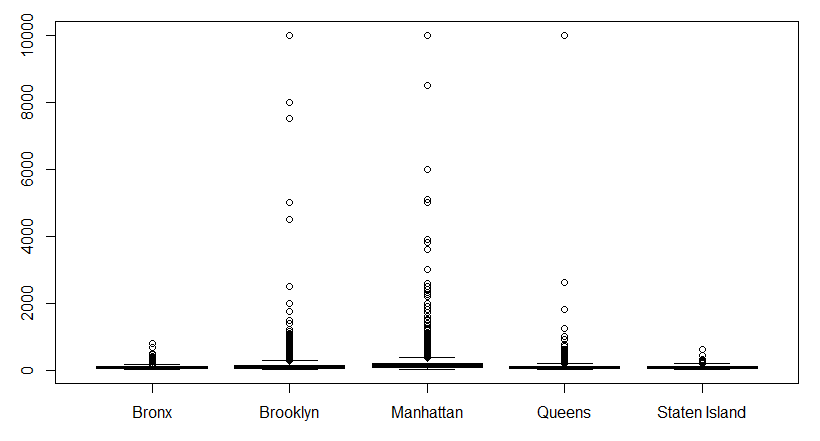
\includegraphics[width=8cm]{neighborhood_grp_corr.png}
			\centering
			\caption{Correlation between neighbourhood group and price}
			\label{neighborhood_grp_corr}
		\end{figure}
		\item The room type of the Airbnb listing affects its price. There are three room types in the dataset: Entire home/apartment, Private room, and Shared room. The correlation plot in Figure \ref{room_type_corr} clearly shows that Entire home/apartments are priced higher than private rooms, and Shared rooms are the least expensive of them all.
		\begin{figure}[ht]
			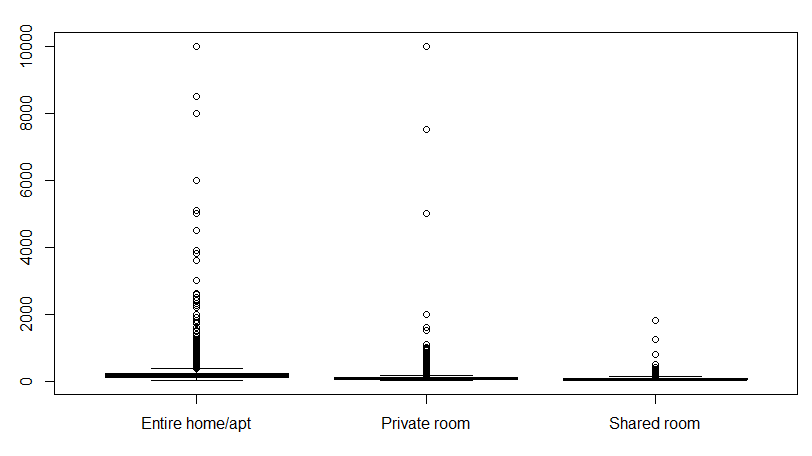
\includegraphics[width=8cm]{room_type_corr.png}
			\centering
			\caption{Correlation between room type and price}
			\label{room_type_corr}
		\end{figure}
		\item The neighbourhood impacts the price of the Airbnb listing as well. From the correlation plot, it is observed that listings in neighbourhoods like "Upper West Side", "Upper East Side", and "Easts Harlem" have a higher price compared to those in other areas. Figure \ref{neighborhood_corr} shows the correlation plot.
		\begin{figure}[ht]
			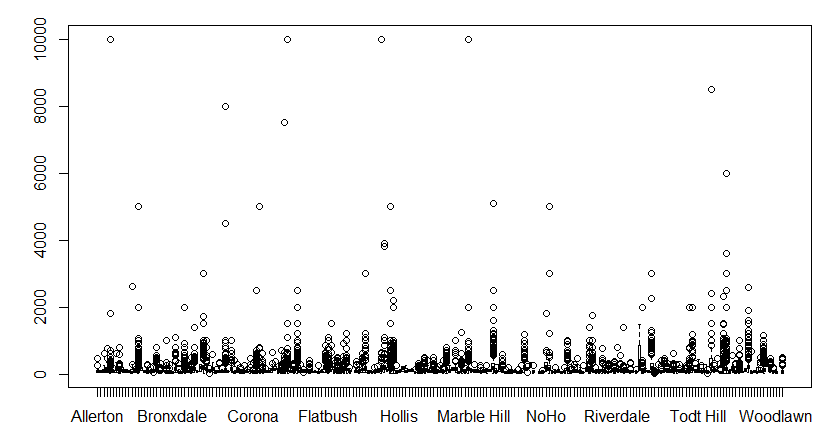
\includegraphics[width=8cm]{neighborhood_corr.png}
			\centering
			\caption{Correlation between neighbourhood and price}
			\label{neighborhood_corr}
		\end{figure}
		\item Some attributes which initially seemed to have business meaning did not have a strong correlation to the price. These attributes are "availability\_365", and "minimum\_nights".
	\end{enumerate}
	Figure \ref{corr} depicts the summary of all the above correlation plots with the price, which will help choose the right features for the model. 
	\begin{figure}[ht]
		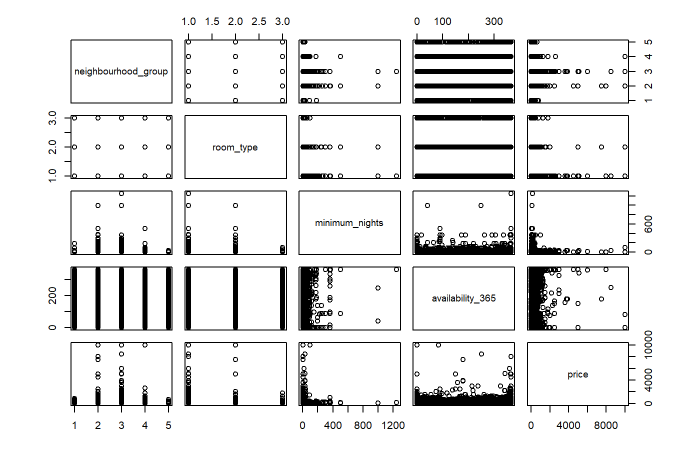
\includegraphics[width=8cm]{corr.png}
		\centering
		\caption{Correlation of price between other attributes}
		\label{corr}
	\end{figure}
	\subsection{Outcomes of Data Exploration and Visualization}
	Data exploration and visualization provided a clear understanding of the type of the data and its quality, which provides a clear idea of the preprocessing steps required to make the data more suitable for the data mining task. These results are briefly described below:
	\begin{description}
		\item[Type of the data:] The attributes that have an impact on the price are of varying types. For example, "neighbourhood" and "neighbourhood\_group" contain discrete values which can be categorized, and "room\_type" is a special categorical attribute where each category carries a meaning of "level" with it. In addition to these, the target label, "price", is itself a continuous attribute which can be categorized given the uneven spread of its values across the records. This can be observed in the histogram in Figures \ref{price_hist_1} and \ref{price_hist_2}
		\begin{figure}[ht]
			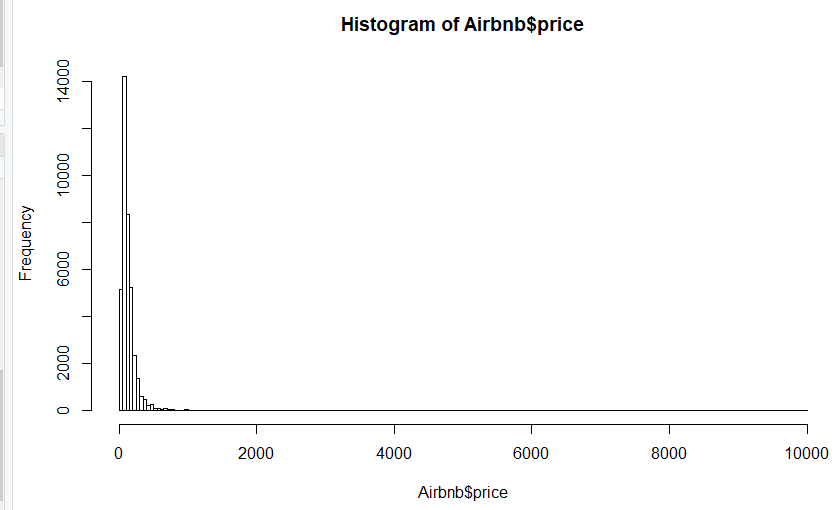
\includegraphics[width=8cm]{price_hist_1.png}
			\centering
			\caption{Distribution of the price}
			\label{price_hist_1}
		\end{figure}
		\begin{figure}[ht]
			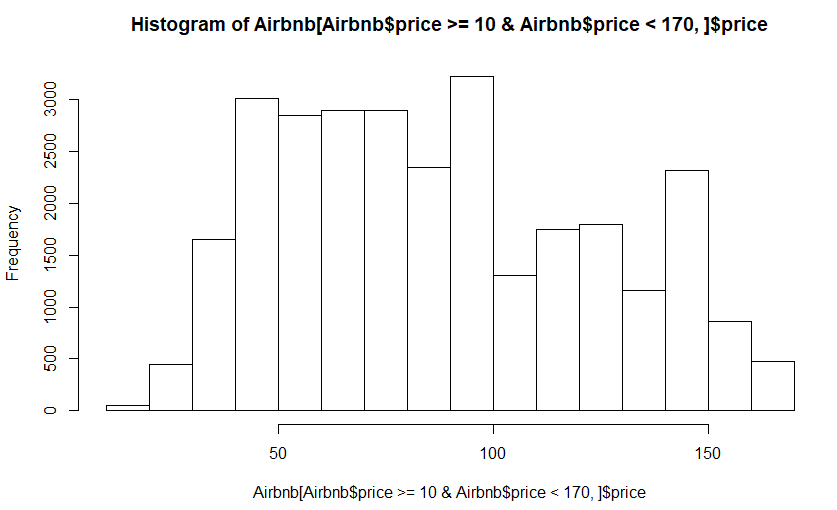
\includegraphics[width=8cm]{price_hist_2.png}
			\centering
			\caption{Distribution of the price between the first and third quantiles}
			\label{price_hist_2}
		\end{figure}
		\item[Quality of the data:] It was observed that the data contains certain records with data missing on attributes that might impact the data mining result, such as "room\_type", and "availability\_365". Also, a few records were found with 0 price. It was decided that these records would be considered spurious, and would be removed from the data fed to the classifier. The summary of price is described in Figure \ref{price_summary}.
		\begin{figure}[ht]
			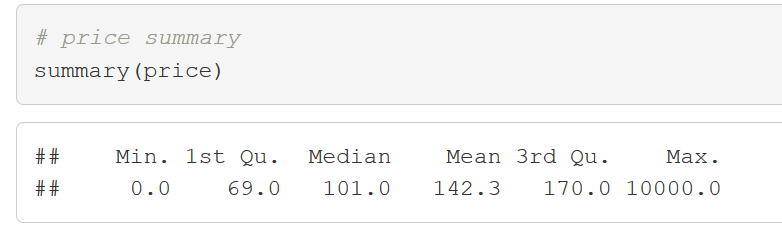
\includegraphics[width=8cm]{price_summary.png}
			\centering
			\caption{Summary, and spurious values for price}
			\label{price_summary}
		\end{figure}
	\end{description}
	
	\section{Categorizing Price}
	Price the New York Airbnb Dataset is a continuous attribute with the following details - \newline
	Min.   :    10.0  \newline
	1st Qu.:   69.0  \newline
	Median :  101.0  \newline
	Mean   :  141.8  \newline
	3rd Qu.:  170.0  \newline
	Max.   :10000.0  \newline
	To perform a classification task on the price, this attribute has to be made categorical. We used quartiles to create four different classes ranging from cheap to expensive. The quartiles were as follows,
	Category 1 : 25\% (10 - 69) \newline
	Category 2 : 50\% (70 - 101) \newline
	Category 3 : 75\% (102 - 170) \newline
	Category 4 : 100\% (171 - 10000) \newline
	Figure \ref{dist} shows the distribution of the data after the categorical split. As seen below, the distribution is well balanced with all classes having approximately the same number of instances, eliminating any class skewed dataset problems.
	\begin{figure}[ht]
		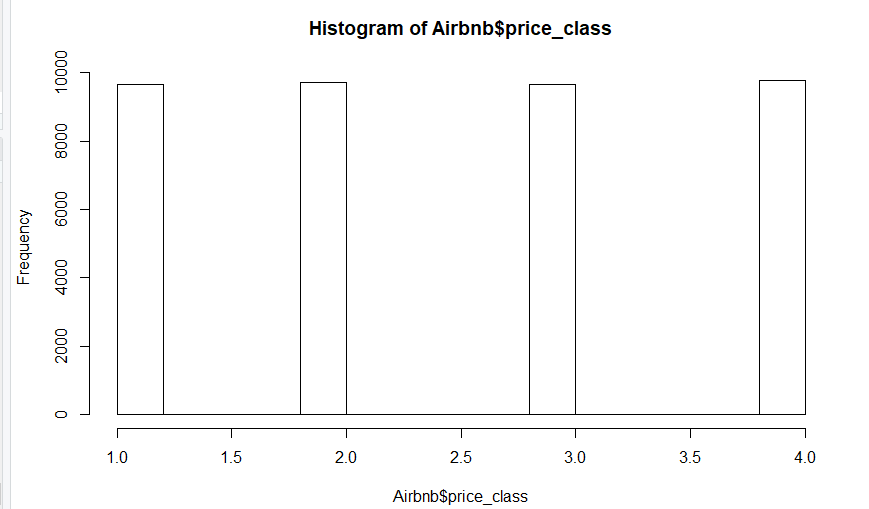
\includegraphics[width=8cm]{dist.png}
		\caption{Distribution of price after categorizing}
		\label{dist}
		\centering
	\end{figure}
	\section{Cleaning the dataset}
	Since the dataset consists of both missing and inconsistent values, the first stage in the data mining process is to clean or eliminate these records.
	The total number of records in the dataset is 48,895 records. 10,052 records had missing values in last\_review and reviews\_per\_month. However, since we foresee some significance in using these attributes to determine price, these missing records have to be eliminated to prevent incorrect data. The size of the dataset after eliminating the missing values is 38,843 records.
	Further, there are 10 records in the dataset that have the price value as 0. While these data records may be accurate, they form outliers that can interfere with the model's accuracy. 
	The final dataset consists of 38,833 records. 
	\section{Feature Engineering} 
	\subsection{Dimensionality Reduction}
	In an attempt to reduce the dimensions of the dataset, attributes that are unlikely to contribute to the prediction of the price group without intensive preprocessing are eliminated. For instance, while the host name and the description of the listing could indirectly contribute to the price (An unknown pattern that could reveal that customers are more likely to pick a specific listing based on description - old ancient house versus new house in the suburb), these features are not easily found through simple classification techniques. 
	\subsection{Factoring attributes}
	Factoring attributes allows R to encode the vector (in this case, the attribute column) into a categorical attribute. For the attributes room type, neighborhood, neighborhood group are all categorical values and hence these are factored to make them understandable to an R algorithm. The attribute availability 365 is a real valued number. Since this value would not easily be used to make a decision tree split, the attribute is split into 3 bins based on the 33rd and 66th percentile and then factored.  
	\subsection{Leveling attributes}
	Leveling an attribute in R allows categorical attributes to be ordered in a meaningful manner. For instance, the attribute room type is ordered for 3 levels.
	\begin{itemize}
		\item Level 1 - Shared room
		\item Level 2 - Private room
		\item Level 3 - Entire home/apartment
	\end{itemize}
	
	\section{Train and test split}
	The final stage of the preprocessing is splitting the dataset into train and test in a 80-20 ratio. The dataset is shuffled to ensure that there is representation of the data distribution in both the parts. As seen in figures \ref{trainhist} and \ref{testhist}, the distribution for all categories of price group remains the same in both train and test. All models that will be built will use train and test accuracy as a metric to determine performance. These accuracy measures will also be used to identify potential problems such as overfitting and underfitting if they occur and in turn work towards a model that eliminates such issues.  
	\begin{figure}[ht]
		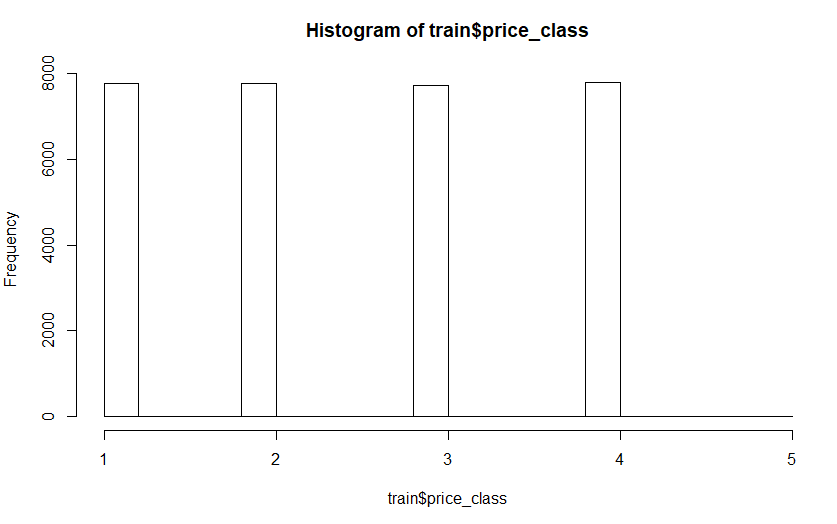
\includegraphics[width=8cm]{trainhist.png}
		\caption{Distribution of price in Train}
		\label{trainhist}
		\centering
	\end{figure}
	\begin{figure}[ht]
		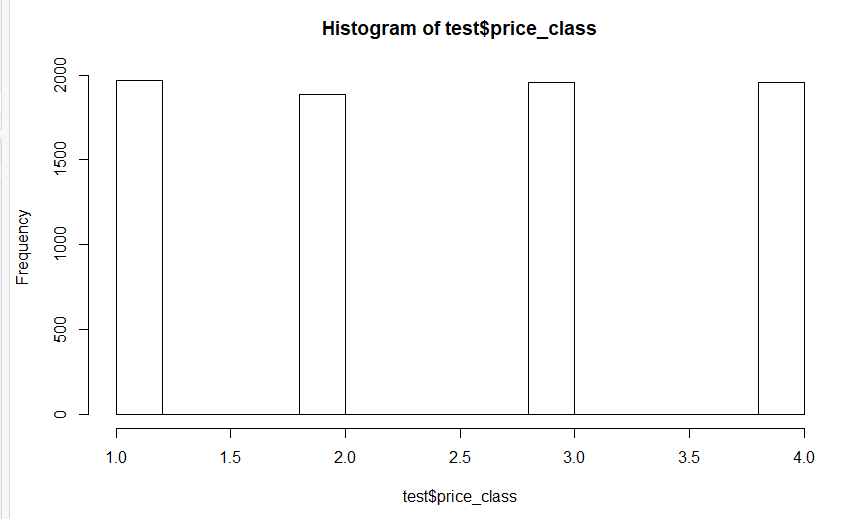
\includegraphics[width=8cm]{testhist.png}
		\caption{Distribution of price in Test}
		\label{testhist}
		\centering
	\end{figure}
	\section{Choosing the classification model}
	The next phase involved trying three different classification models to determine which one is more effective in modeling the dataset. The three considered were decision trees, K nearest neighbors, and Naive Bayes algorithm. \\
	For the purpose of testing with the raw dataset but still performing a classification tasks, the following modifications were made to the dataset.\\
	\begin{itemize}
		\item The outliers in the price column were eliminated and price was split into two categories - no more than 100 and greater than 100.
		\item Only attributes with numerical values that required no preprocessing were used
		\item The train and test split ratio was 9:1.
	\end{itemize}
	The three algorithms were fitted to this dataset using R and the following documents the results obtained from the same.
	\begin{itemize}
		\item Decision Tree : Accuracy 72\%
		\item K Nearest Neighbors : Accuracy 64\% (k =20)
		\item Naive Bayes : Accuracy 68\%
	\end{itemize}
	\begin{figure}[ht]
		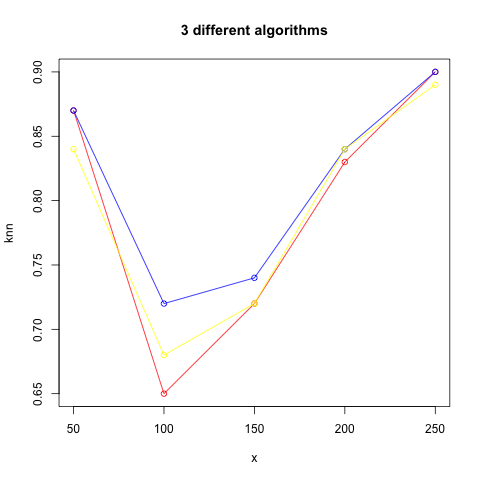
\includegraphics[width=8cm]{line_diagram.jpg}
		\caption{Accuracy performance - Decision Tree (Blue), Naïve Bayes (Yellow), kNN (Red)}
		\label{linediag}
		\centering
	\end{figure}
	
	Figure \ref{linediag} depicts the performance of all three algorithms on the dataset. Through these results, we conclude that the decision tree algorithm is the most suitable for the New York Airbnb dataset and the next phase will be using only this algorithm.
	\section{The Decision Tree} 
	A decision tree is constructed on the resulting data from our preprocessing stage. To summarize, the tree uses the attributes listed below to predict the outcome of the price group (ranges from 1 to 4)
	\begin{itemize}
		\item Neighbourhood
		\item Neighbourhood group
		\item Room type
		\item Minimum nights
		\item Number of reviews
		\item Number of listings by host
		\item Reviews per month
	\end{itemize}
	The decision tree is built using the rpart model available from R. RPart stands for Recursive Partitioning And Regression Trees and requires only one compulsory parameter to build the model. \newline
	Formula : This parameter indicates the value to be predicted and all the attributes that must be used to predict it\newline
	\subsection{Refining the decision tree using preprocessed data}
	\begin{itemize}
		\item Our first decision tree is built on only the raw categorical data to see how the model performs.\\
		The categorical attributes used for this is the neighbourhood group and the room type. \\
		Figure \ref{decision1} depicts the decision tree built using only categorical data. Its accuracy is at 51.95056\%.
		\begin{figure}[ht]
			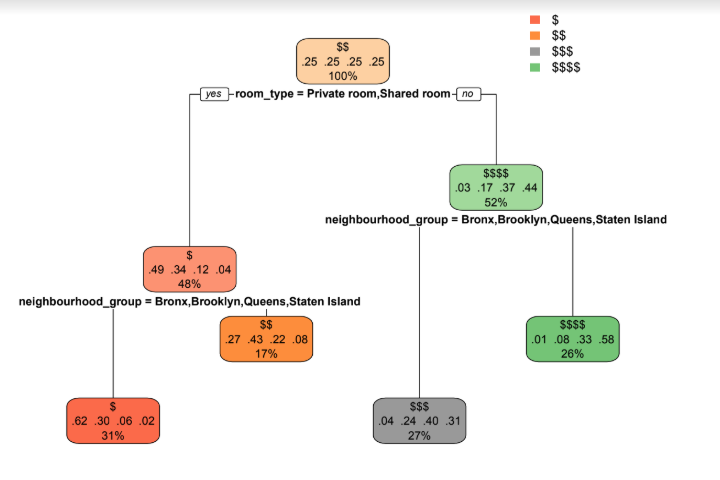
\includegraphics[width=8cm]{decision1.PNG}
			\caption{Decision tree with only categorical attributes}
			\label{decision1}
			\centering
		\end{figure}
	\item In an attempt to improve this performance, we convert the numerical data into appropriate categorical values and build a new decision tree.\\
	The latitude attribute is divided into North and South, the longitude into East and West.\\
	Figure \ref{decision2} depicts the decision tree built with these additions. Its accuracy is 52.98056\%.
	\begin{figure}[ht]
		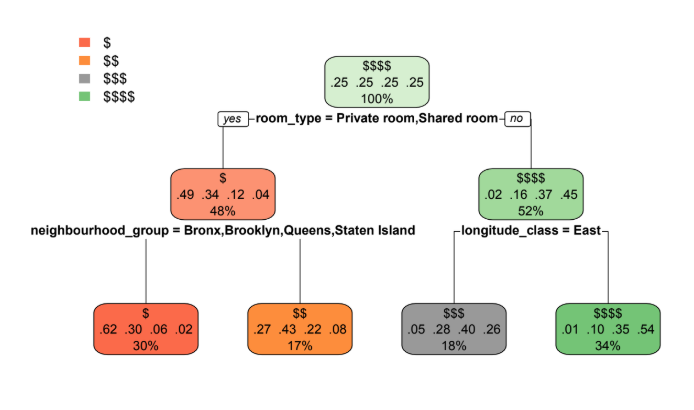
\includegraphics[width=8cm]{decision2.PNG}
		\caption{Decision tree with categorical and numerical attributes}
		\label{decision2}
		\centering
	\end{figure}
	\item The next step in improving the performance of the decision tree is the cleaning the current data to remove any outliers or meaningless values. These changes affect the attributes minimum nights, availability\_365 and host listing count\\
	Further, on visualization of the attributes, we noticed that the east and west classes were not balanced as seen in figure \ref{longsplit} and hence we shifted the split towards the east class in an attempt to balance the classes\\
	Figure \ref{decision3} depicts the decision tree built with these additions. The accuracy of the tree built after these changes is 54.01713\%
	\begin{figure}[ht]
		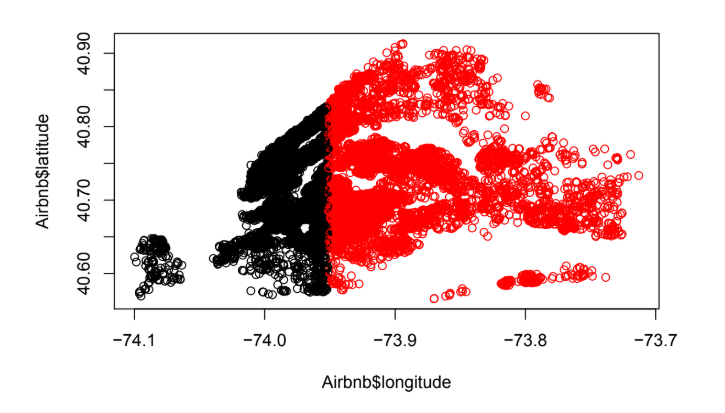
\includegraphics[width=8cm]{longsplit.PNG}
		\caption{Plot of longitude split on New York Map}
		\label{longsplit}
		\centering
	\end{figure}
	\begin{figure}[ht]
		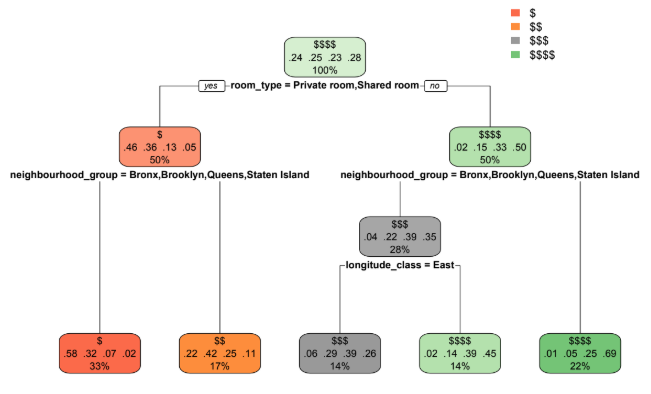
\includegraphics[width=8cm]{decision3.PNG}
		\caption{Decision tree after cleaning outliers}
		\label{decision3}
		\centering
	\end{figure}
	\end{itemize}
	\subsection{Refining the price split}
	The next attempt in improving the model's performance was by changing the price split. So far, the price was discretized into four categories based on quantiles. In this stage, the real values are categorized into 3 classes based on percentile - 0, 0.33, 0.66. All the remaining attributes are left unchanged and the decision tree is built.\\
	Figure \ref{decision4} depicts the decision tree built on the three way split. We note that this change positively impacts the accuracy and brings it up to 66.6821\%
	\begin{figure}[ht]
		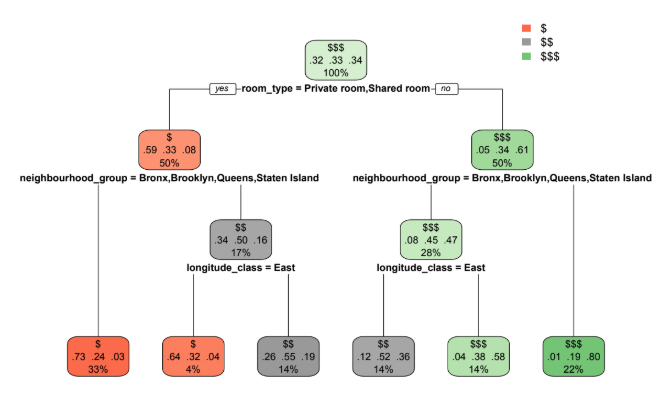
\includegraphics[width=8cm]{decision4.PNG}
		\caption{Decision tree with three way price split}
		\label{decision4}
		\centering
	\end{figure}
	\subsection{Adding more attributes from another dataset}
	Airbnb is a publicly available dataset that contains even more features compared to the New York Airbnb dataset that we are currently using. To explore these features and see if they are good predictors for the price class, we merge the two datasets based on their unique name and id. \\
	The new features obtained from this merge including the cleaning fee and the cancellation policy. Figure \ref{cancellation} show the distribution of these attributes. 
	The cleaning fee is a real valued attribute and is hence categorized based on percentile into three classes.\\
\begin{figure}[ht]
	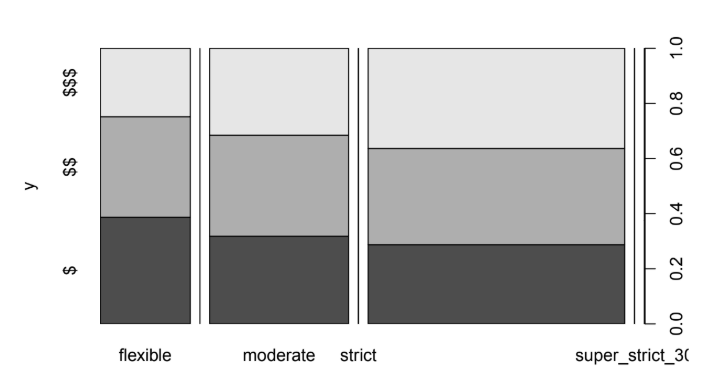
\includegraphics[width=8cm]{cancellation.PNG}
	\caption{Cancellation Policy Distribution based on price}
	\label{cancellation}
	\centering
\end{figure}
	The decision tree for the three way price split is then built with these new attributes also added to the formula. Figure \ref{decision5} is the result of this change.\\
	However, we notice that the additional features do not positively impact the accuracy. In fact, the accuracy after these changes is at 54.54545\%
	\begin{figure}[ht]
		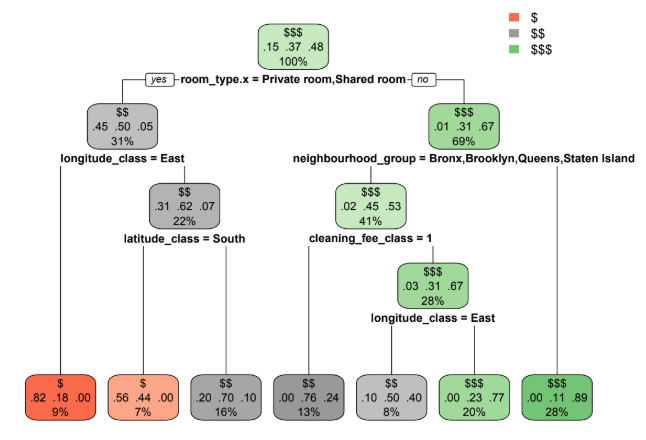
\includegraphics[width=8cm]{decision5.PNG}
		\caption{Decision tree with more attributes}
		\label{decision5}
		\centering
	\end{figure}
	\section{Results}
	Figure \ref{nyheatmap} depicts our predictions across the New York map. As we can see, most of the state is expensive with few regions that fall into the lower price categories which fits in with the ground truth.\\ 
	\begin{figure}[ht]
		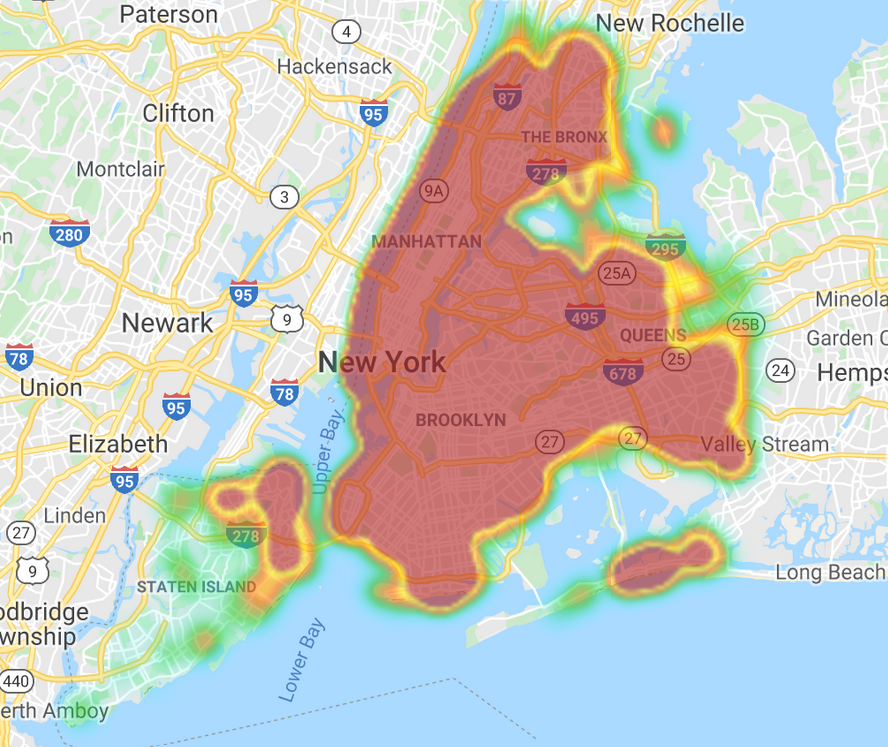
\includegraphics[width=8cm]{heatmap.png}
		\caption{Heat Map of the Price Class Predictions}
		\label{nyheatmap}
		\centering
	\end{figure}	
\end{document}
